\documentclass[a4paper, 12pt]{article}
\usepackage[a4paper,top=1.5cm, bottom=1.5cm, left=1cm, right=1cm]{geometry}
\usepackage{cmap}					
\usepackage{mathtext} 				
\usepackage[T2A]{fontenc}			
\usepackage[utf8]{inputenc}			
\usepackage[english,russian]{babel}
\usepackage{multirow}
\usepackage{graphicx}
\usepackage{wrapfig}
\usepackage{tabularx}
\usepackage{float}
\usepackage{longtable}
\usepackage{hyperref}
\hypersetup{colorlinks=true,urlcolor=blue}
\usepackage[rgb]{xcolor}
\usepackage{amsmath, amsfonts, amssymb, amsthm, mathtools} 
\usepackage{icomma} 
\usepackage{euscript}
\usepackage{mathrsfs}
\usepackage{enumerate}
\usepackage{caption}
\usepackage{enumerate}
\mathtoolsset{showonlyrefs=true}
\usepackage{graphicx}
\usepackage{caption}
\usepackage{subcaption}
\usepackage{amsthm}
\usepackage{floatflt}
\usepackage[europeanresistors, americaninductors]{circuitikz}
\DeclareMathOperator{\sgn}{\mathop{sgn}}
\newcommand*{\hm}[1]{#1\nobreak\discretionary{}
	{\hbox{$\mathsurround=0pt #1$}}{}}

\title{\textbf{Петля гистерезиса (статический метод) (3.4.4)}}
\author{Манро Эйден}
\date{}

\begin{document}

\maketitle

\noindent \textbf{Цель работы:} Исследование кривых намагничивания ферромагнетиков с помощью баллистического гальванометра.

\bigskip

\noindent \textbf{В работе используются:} генератор тока с блоком питания, тороид, соленоид, баллистический гальванометр с осветителем и шкалой, амперметры, магазин сопротивлений, лабораторный автотрансформатор (ЛАТР), разделительный трансформатор.

\section*{Теоретические положения}

\begin{floatingfigure}{41mm}
\noindent
\hfil
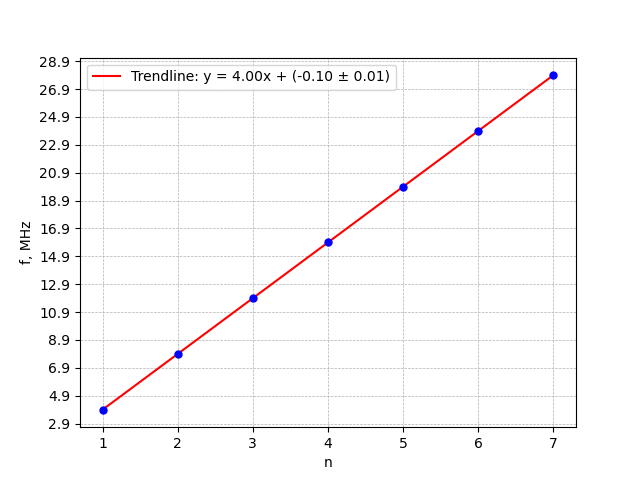
\includegraphics[width=41mm]{fig1.PNG}
\hfil
\caption{Петля гистерезиса ферромагнетика}
\label{figCurvesFF}
\end{floatingfigure}

Магнитная индукция \textbf{B} и напряжённость магнитного поля \textbf{H} в ферромагнетике неоднозначно связаны между собой: индукция зависит не только от напряжённости, но и от предыстории образца. В эксперименте будет исследоваться \textit{основная кривая намагничивания OACD} и \textit{предельная петля гистерезиса DEFD'E'F'D} (см. рис. 1).

С помощью баллистического гальванометра и амперметра будем косвенно измерять зависимость индукции магнитного поля от его напряжённости. \\
Напряжённость магнитного поля \textit{Н} в тороиде зависит от тока, текущего в намагничивающей обмотке:
\begin{equation}
    H = \frac{N_{T_0}}{\pi D}I,
\end{equation} 
где $D$ - средний диаметр тора, $N_{T_0}$ - количество витков.

Изменение поля приводит к изменению потока магнитной индукции Ф в сердечнике, в измерительной обмотке возникает ЭДС индукции, через гальванометр, в свою очередь, протекает импульс тока, изменяется положение рамки и, следовательно, зайчика. Окончательно (определив также баллистическую постоянную гальванометра, проведя измерения с соленоидом) для изменения магнитной индукции в сердечнике тороида получаем:

\begin{equation}
    \triangle B = \mu_0 (\frac{d_C}{d_T})^2 \frac{R}{R_1} \frac{N_C_0}{N_T_1} \frac{N_C_1}{l_C} \triangle I_{c} \frac{\triangle x}{\triangle x_{c}},
\end{equation}
где $R$ - полное сопротивление измерительной цепи тороида, $d_C, d_T$ - диаметр поперечного сечения соленоида и тороида соответственно, $N_C_0$  - число витков пустотелого соленоида, $N_C_1$ - число витков короткой измерительной катушки $l_C$ - длина соленоида, $\triangle x_c$ - отклонение зайчика при работе с соленоидом, $\triangle x$ - отклонение зайчика в эксперименте, $\triangle I_{c}$ - ток соленоида.

Также нам понадобится максимальная дифференциальная магнитная проницаемость 
\begin{equation}
    \mu_{diff} = \frac{1}{\mu_0}\frac{dB}{dH}
\end{equation}

характеризующяя связь между магнитной индукцией B и напряжённостью магнитного поля H в веществе.

\newpage

\section*{Экспериментальная установка}

\begin{figure}[H]
    \centering
    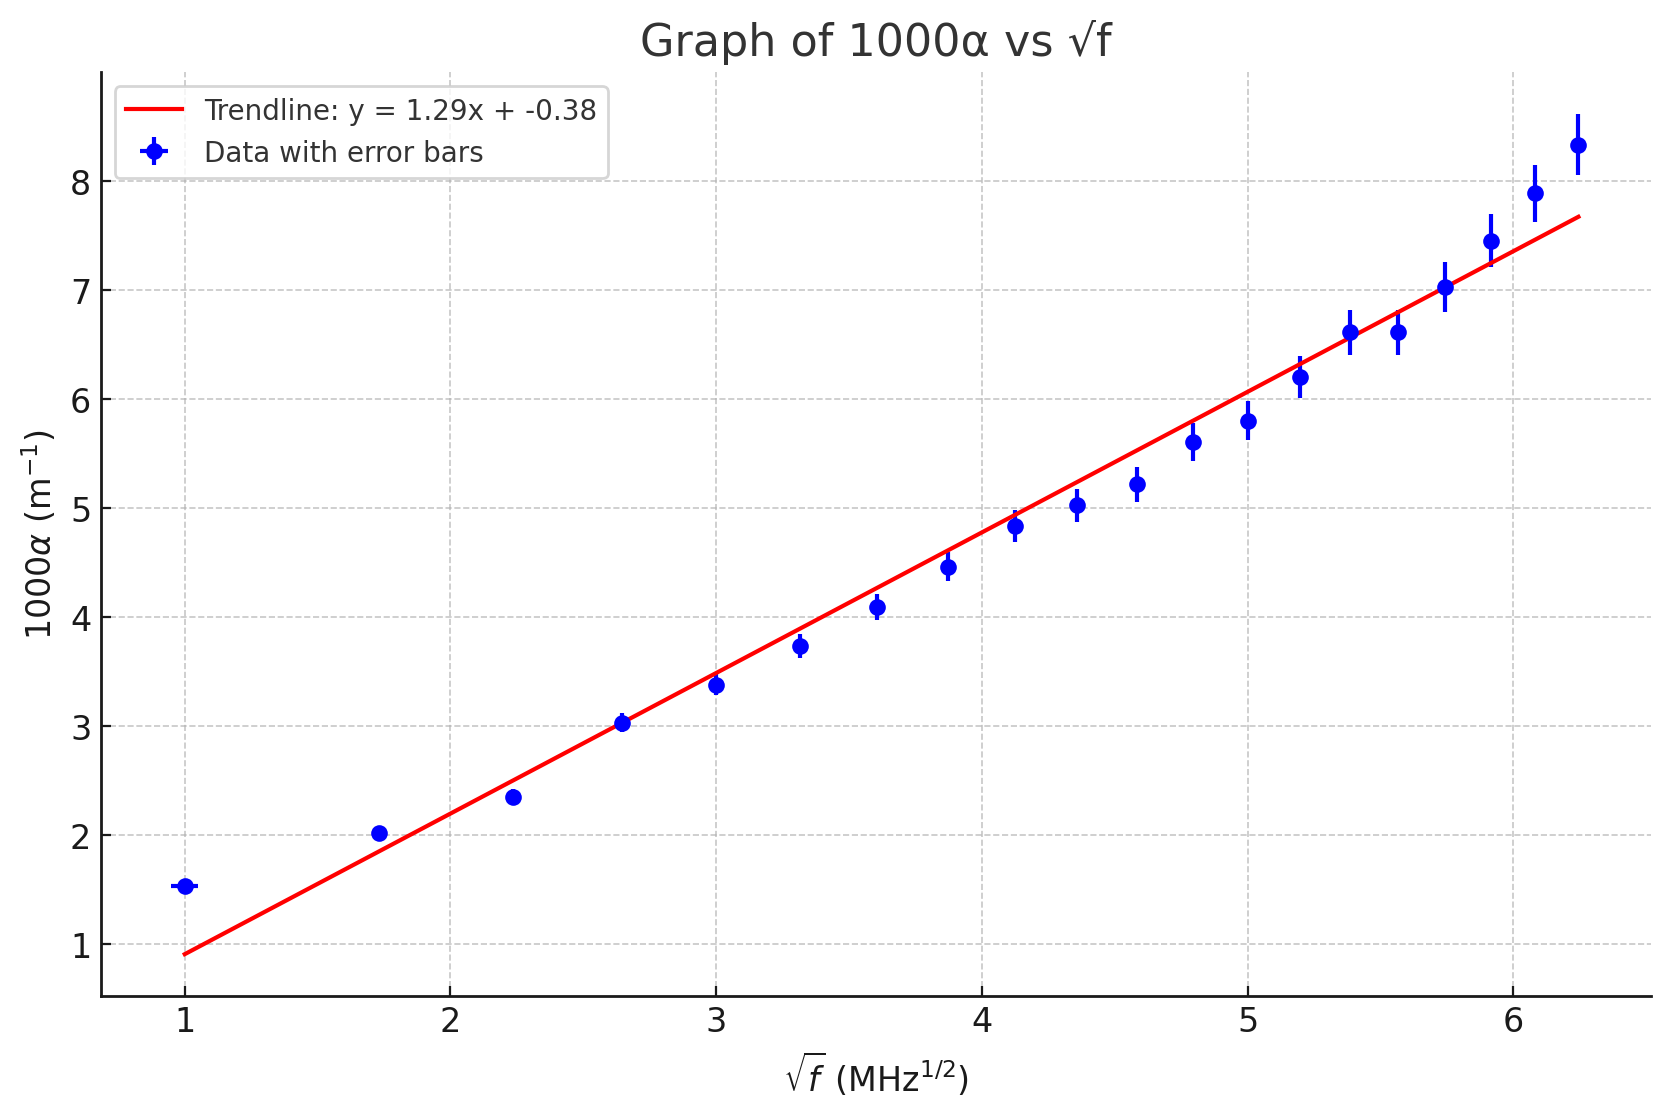
\includegraphics[width=10cm]{fig2.PNG}
    \caption{Схема установки для исследования петли гистерезиса}
    \label{fig:vac}
\end{figure}

\begin{figure}[H]
    \centering
    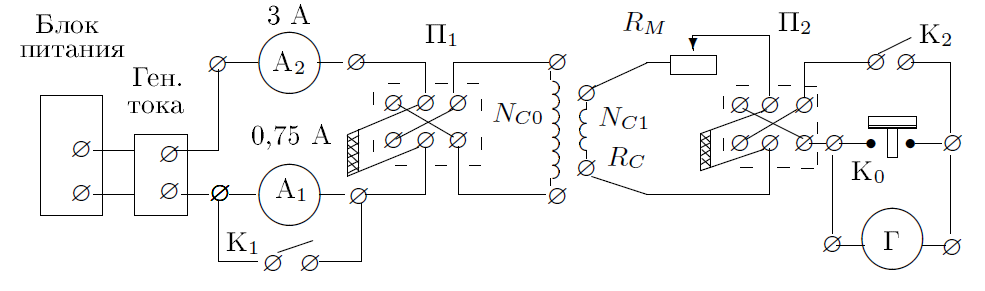
\includegraphics[width=10cm]{fig3.PNG}
    \caption{Схема установки для калибровки гальванометра}
    \label{fig:vac}
\end{figure}

После снятия петли гистерезиса необходимо размагнитить сердечник, подключив его к цепи переменного тока, постепенно снижая его амплитуду. Только затем следует приступать к снятию основной кривой намагничивания.

\section*{Результаты}

\begin{figure}[ht]
    \centering
    \begin{minipage}[b]{0.45\linewidth}
        \centering
        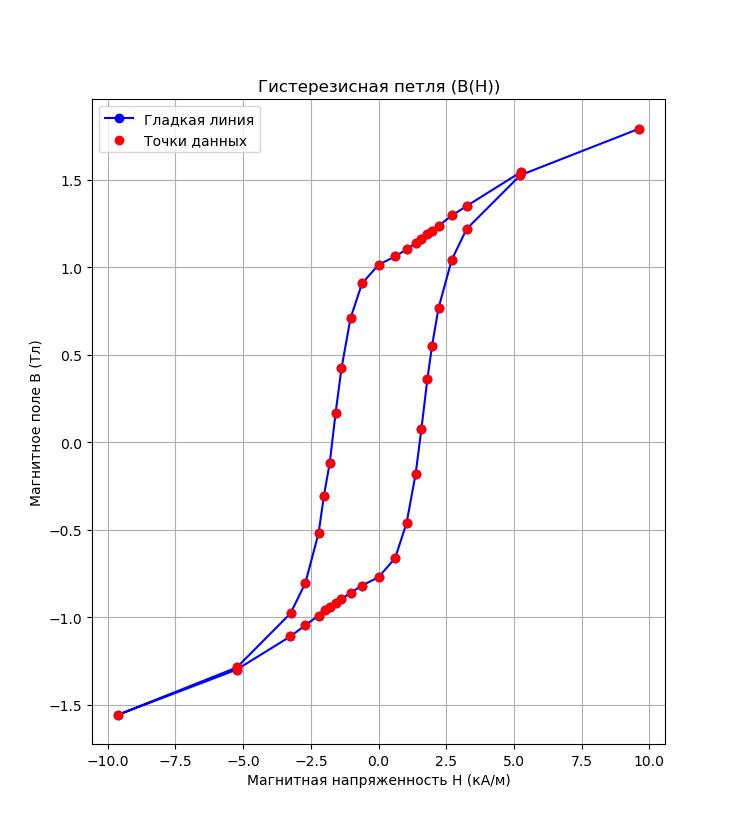
\includegraphics[width=1.1\linewidth]{fig1_no_errors.png}
        \caption{Гистерезис}
        \label{fig:graph1}
    \end{minipage}
    \hfill
    \begin{minipage}[b]{0.45\linewidth}
        \centering
        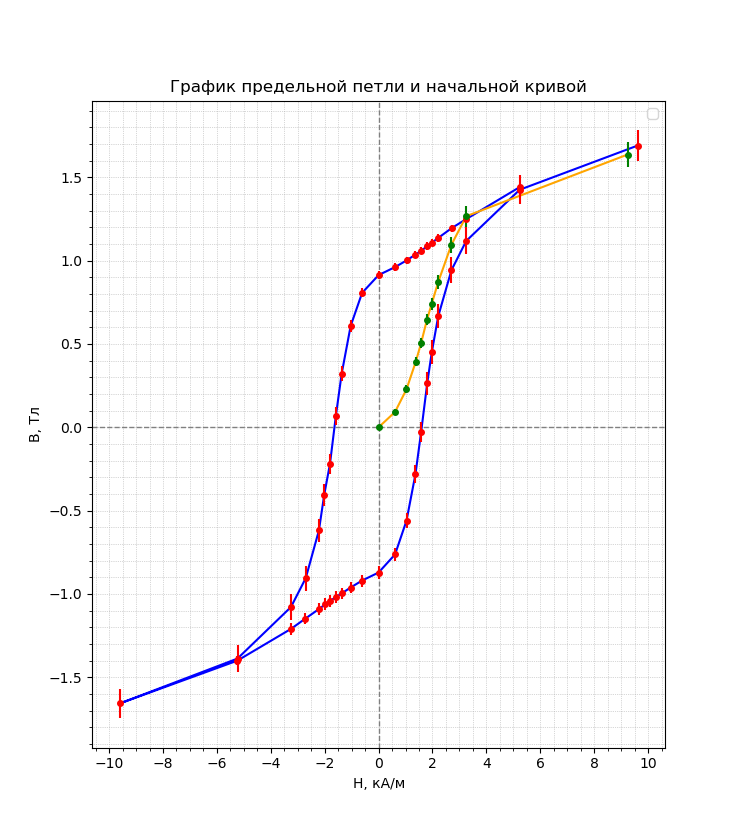
\includegraphics[width=1.1\linewidth]{fig2_with_inital_curve_and_errors.png}
        \caption{Гистерезис и начальная кривая}
        \label{fig:graph2}
    \end{minipage}
    \label{fig:graphs}
\end{figure}

\begin{figure}[H]
    \centering
    \begin{minipage}[b]{0.45\linewidth}
        \centering
        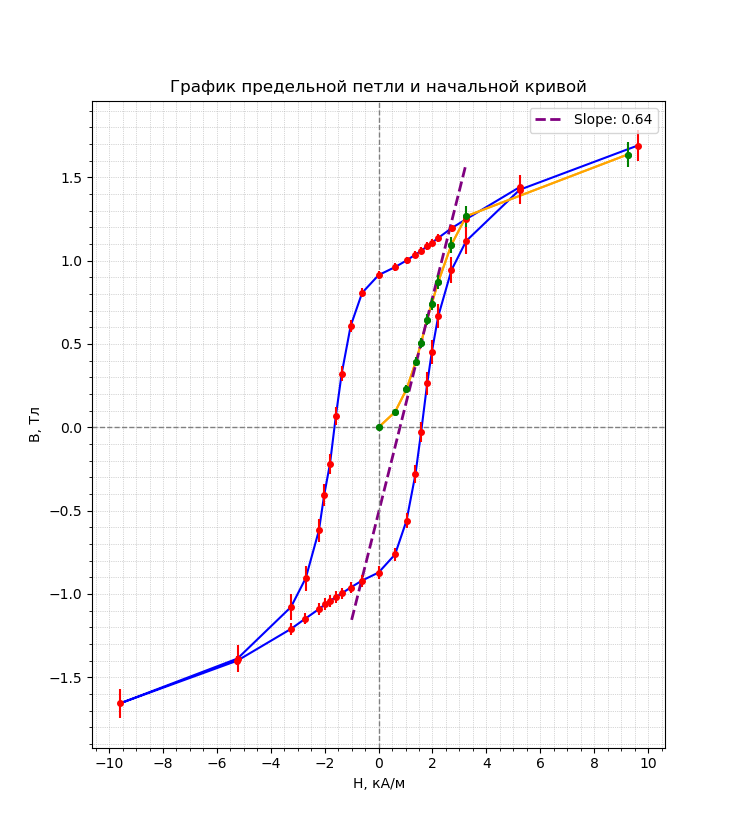
\includegraphics[width=1.2\linewidth]{fig3_with_slope.png}
        \caption{Гистерезис c прямой максимального наклон}
        \label{fig:graph1}
    \end{minipage}
    \hfill
    \begin{minipage}[b]{0.45\linewidth}
        \centering
        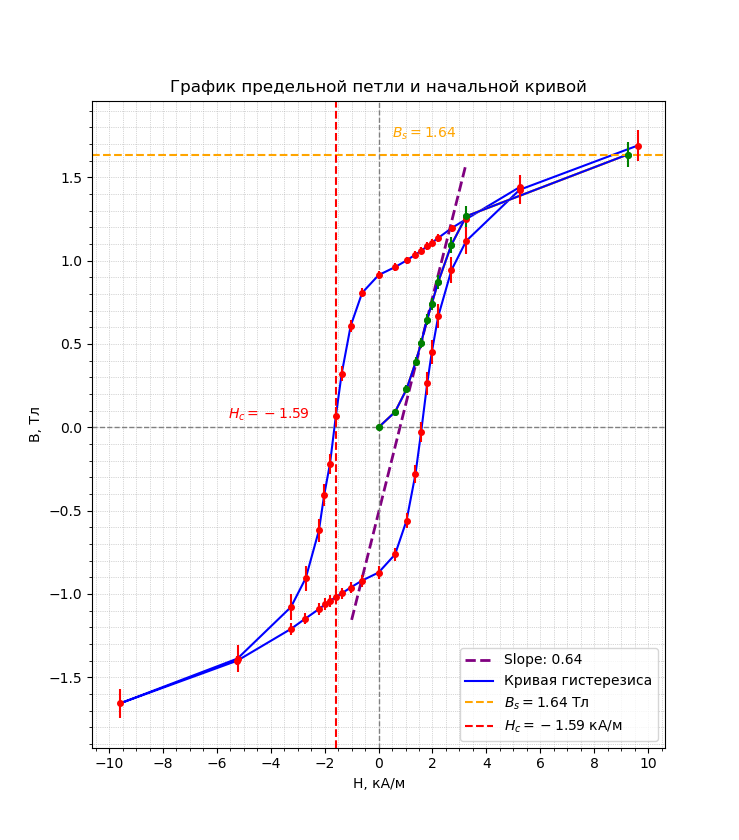
\includegraphics[width=1.2\linewidth]{fig4_with_bars.png}
        \caption{Гистерезис с прямой и важными параметрами}
        \label{fig:graph2}
    \end{minipage}
    \label{fig:graphs}
\end{figure}

\begin{itemize}
    \item коэрцитивная сила $H_c$ - значение напряжённости магнитного поля, необходимое для полного размагничивания ферромагнитного вещества равна длине отрезка, высекаемого петлёй гистерезиса на горизонтальной оси. 
    \begin{equation}
        H_c = 1.59 \pm 0.02 \; \text{кА/м}
    \end{equation}
    \item индукция насыщения $B_s$ -  максимально достижимое значение внутренней индукции магнитного материала при данной температуре. 
    \begin{equation}
        B_s = 1.6 \pm 0.1 \; \text{Тл}
    \end{equation}
    \item максимальная дифференциальная магнитная проницаемость $\mu_d = \frac{1}{\mu_0}\frac{dB}{dH}$ - характеризующий связь между магнитной индукцией B и напряжённостью магнитного поля H в веществе. 
    \begin{equation}
        \mu_{d} = 510 \pm 10
    \end{equation}
\end{itemize}

\section*{Вывод} 
В ходе работы были исследованы петля гистерезиса магнитомягкого материала, его начальная кривая намагничивания, с хорошей точностью экспериментально определены некоторые магнитные свойства. В нашем случае тор был изготовлен из стали. Для обычной углеродной стали дифференциальная проницаемость может находиться в пределах от 100 до 1000. Так что можно сказать, что с материалом нас не обманули. Сталь обладает низким уровнем гистерезиса и высокой магнитной проницаемостью. Такие материалы быстро намагничиваются и размагничиваются, что делает их идеальными для использования в устройствах, где требуется частое переключение магнитных полей, например, в трансформаторах, электродвигателях и других электрических аппаратах.

\end{document}